\begin{document}
%=================================================================
%                           Start Document
%=================================================================
\section{Implementation}
\lhead{Implementation} % section header
\setstretch{1.6}
\lhead{Implementation - Software Refactoring}
\subsection{Software Refactoring}
As mentioned introduction wise this project builds upon the work and code base originally developed for FES with the LegoPress \cite{olivier_legopress_2014} and further developed by a previous student. However the code quality was poor with thousands of lines of code and multiple functionalities all implemented in one file and one class. Therefore before continuing on with the project a proper refactoring of the code was necessary. The goal being to save time in the long run by creating modular, robust, readable code that could later be further built upon for use in clinical trials.

The software is written in C++ in QT.

\subsubsection{Documentation}

In order to understand the code it was decided that the first step would be to create documentation, specifically graphical representations of the interactions and hierarchy. To accomplish the code was documented and edited so that it would be compatible with doxygen. Doxygen is a documentation generation tool that automatically creates software documentation from annotated source code in HTML.

\begin{figure} [H]
    \centering
    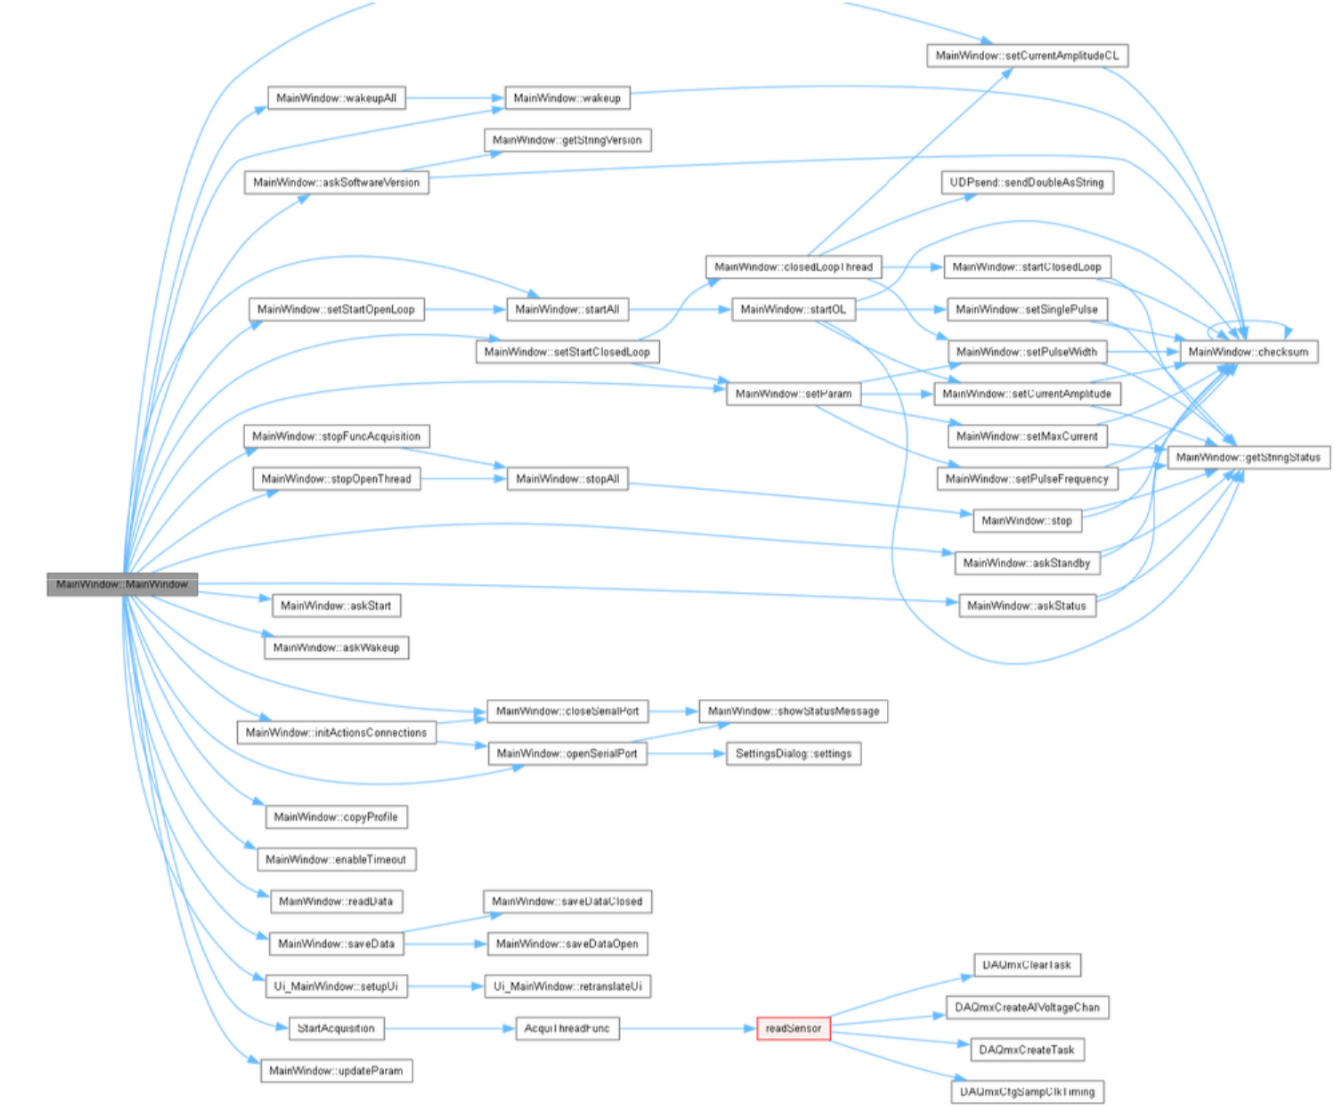
\includegraphics[width=0.9\linewidth]{images/oldDoxy.png}
    \caption{Original callgraph for mainwindow function before refactoring, generated by doxygen}
    \label{fig:oldDoxy}
\end{figure}

After the code had been documented and visualized in doxygen it became possible to see the call graphs and interactions such as in figure \ref{fig:oldDoxy}. This sped up the process of understanding the code thus laying important groundwork for the clearning and modularization step.

\subsubsection{Modularization}
In order to improve the code quality, a modularization and cleaning of the code base was necessary. The code was refactored and divided into classes based mainly on the code quality principles laid out in Code Complete by Steve McConnel \cite{steve_mcconnell_code_nodate}. This includes having clearly defined, minimal interfaces. This is accomplished by using the signal slot mechanism inbuilt into QT, which allows for communication between objects in an event-driven, decoupled manner. Another core concept is organizing modules hierarchically, where higher-level modules depend on lower-level modules but not the reverse. 

\begin{figure} [h]
    \centering
    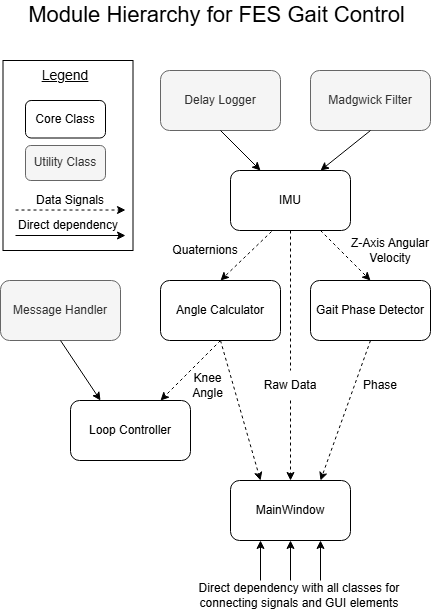
\includegraphics[width=0.6\linewidth]{images/gaitcontrol.png}
    \caption{Module hierarchy after refactoring}
    \label{fig:modulehier}
\end{figure}

A visualization of the hierarchy after refactoring can be seen in figure \ref{fig:modulehier} and description of each class are in table \ref{tab:class-overview}. Previously, all loop controller and IMU functionality and serial communication and bit handling was all done in the mainwindow class. There was also code only relevant for the legopress still in the mainwindow class. That code for the legopress was removed and the usable, existing code was moved to their appropriate classes which were the message handler, LoopController and MainWindow. All old IMU functionality was also removed since part of the project involved changing out the old wired IMUs with the new wireless IMUs developed in the lab. The final architecture has a high cohesion and low coupling resulting in readable, scalable, testable and reusable code.


\lhead{Implementation - Functional Electrical Stimulation Setup}
\subsection{Functional Electrical Stimulation Setup}

\subsubsection{Hardware}
The hardware used for the functional electrical stimulation was the StimWave3


The setup for the functional electrical stimulation consists of the StimWave3 hardware developed at the REHassist lab 


Before moving on to implementing open and closed loop systems for the gait, some changes 



%=================================================================
%                           End Document
%=================================================================
\end{document}